\newpage
\section{Radial velocity with horizontal connection}

\subsection*{Resources}
\begin{itemize}
    \item Book sections 7/1 to 7/5
\end{itemize}

\emph{Correction to book: Figure 7/9 should read $\bm{\alpha} = \bm{\dot{\omega}} = \bm{\Omega} \bm{\times} \bm{\omega}$ (not $\bm{\Omega} \bm{\times} \bm{r}$)}

\subsection*{Challenge}
A weight ``A'' is tethered to a pole by a stiff rod of length $r$. If the angular velocity is \SI{5.5}{\radian\per\second} $\hat{k}$ and the length of the rod is \SI{47}{\meter} along the x-axis, what is the linear velocity of the weight ``A''?

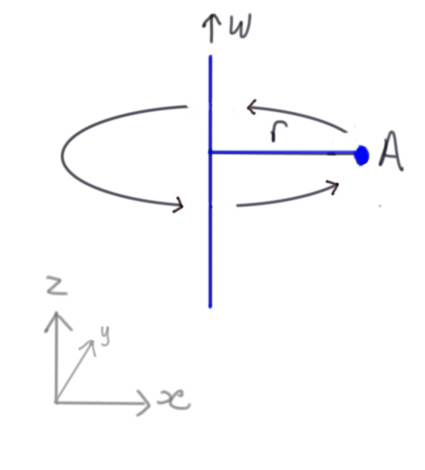
\includegraphics[height=5cm]{rod-horizontal}

\subsection*{Solution}
X = Your solution\\
Units: \si{\meter\per\second}\\
Form: Decimal, to 1 decimal place\\
Place the indicated letter in front of the number\\
Example: aX where $X=42.5$ \si{\meter\per\second} is entered as \href{http://www.wolframalpha.com/input/?i=md5+hash+of+\%22a42.5\%22}{a42.5}

$\hat{i}=$ hash of aX = 9497cd \si{\meter\per\second}\\
$\hat{j}=$ hash of bX = d17e5c \si{\meter\per\second}\\
$\hat{k}=$ hash of cX = 347133 \si{\meter\per\second}




\newpage
\section{Radial velocity with non-horizontal connection}

\subsection*{Resources}
\begin{itemize}
    \item Book sections 7/1 to 7/5
\end{itemize}

\emph{Correction to book: Figure 7/9 should read $\bm{\alpha} = \bm{\dot{\omega}} = \bm{\Omega} \bm{\times} \bm{\omega}$ (not $\bm{\Omega} \bm{\times} \bm{r}$)}

\subsection*{Challenge}
1. The position of ``A'' and the pole are unchanged (the radial distance is the same) and the angular velocity remains the same, but ``A'' is now hinged to the pole from below instead of horizontally, as shown in the picture. Calculate the linear velocity of ``A'' (calculate mathematically, not just by comparison with the previous challenge).

2. Write a sentence or two comparing your answer with that obtained from the previous challenge, including reasoning why.

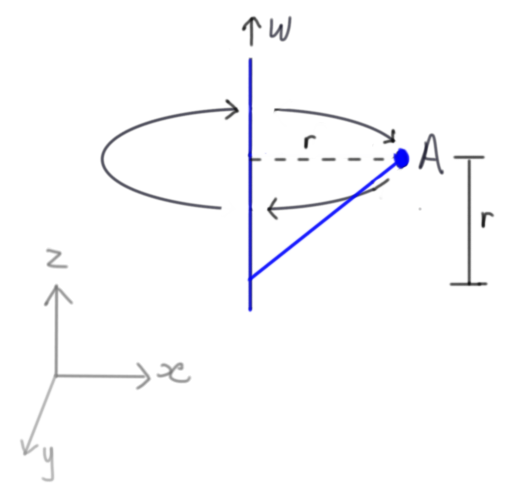
\includegraphics[height=5cm]{rod-frombelow}

\subsection*{Solution}
1.\\
X = Your solution\\
Units: \si{\meter\per\second}\\
Form: Decimal, to 1 decimal place\\
Place the indicated letter in front of the number\\
Example: aX where $X=42.5$ \si{\meter\per\second} is entered as \href{http://www.wolframalpha.com/input/?i=md5+hash+of+\%22a42.5\%22}{a42.5}

$\hat{i}=$ hash of dX = c6e675 \si{\meter\per\second}\\
$\hat{j}=$ hash of eX = bcff19 \si{\meter\per\second}\\
$\hat{k}=$ hash of fX = 979ed8 \si{\meter\per\second}

2. Please discuss in class if you are unsure about your answer.




\newpage
\section{Linear acceleration}

\subsection*{Resources}
\begin{itemize}
    \item Book sections 7/1 to 7/5
\end{itemize}

\emph{Correction to book: Figure 7/9 should read $\bm{\alpha} = \bm{\dot{\omega}} = \bm{\Omega} \bm{\times} \bm{\omega}$ (not $\bm{\Omega} \bm{\times} \bm{r}$)}

\subsection*{Challenge}
Using information from previous challenges, determine the:

1. Linear acceleration towards the centre of pole.

2. The tangential linear acceleration

3. Is there linear acceleration towards the centre of the pole? Is there tangential linear acceleration? Write a sentence or two to explain why for both cases.

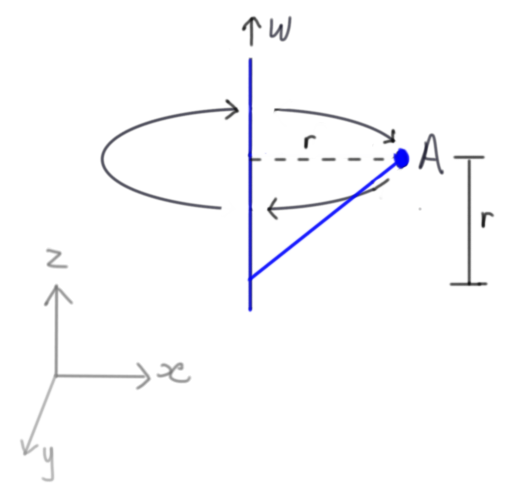
\includegraphics[height=5cm]{rod-frombelow}


\subsection*{Solution}
X = Your solution\\
Units: \si{\meter\per\square\second}\\
Form: Decimal, to 2 decimal place\\
Place the indicated letter in front of the number\\
Example: aX where $X=42.57$ \si{\meter\per\second} is entered as \href{http://www.wolframalpha.com/input/?i=md5+hash+of+\%22a42.5\%22}{a42.57}

1.\\
$\hat{i}=$ hash of gX = e1993f \si{\meter\per\square\second}\\
$\hat{j}=$ hash of hX = 5a16a7 \si{\meter\per\square\second}\\
$\hat{k}=$ hash of iX = 2ebd7c \si{\meter\per\square\second}

2.\\
$\hat{i}=$ hash of jX = 4b3090 \si{\meter\per\square\second}\\
$\hat{j}=$ hash of kX = 28435f \si{\meter\per\square\second}\\
$\hat{k}=$ hash of lX = 060ec3 \si{\meter\per\square\second}

3. Please compare your answer with your partner.




\newpage
\section{Radial acceleration - only magnitude}

\subsection*{Resources}
\begin{itemize}
    \item Book sections 7/1 to 7/5
\end{itemize}

\emph{Correction to book: Figure 7/9 should read $\bm{\alpha} = \bm{\dot{\omega}} = \bm{\Omega} \bm{\times} \bm{\omega}$ (not $\bm{\Omega} \bm{\times} \bm{r}$)}

\subsection*{Challenge}
Now consider that the radial velocity is not constant, but is undergoing an acceleration so that the magnitude of the angular velocity $\bm{w}$ increases while it continues to point in the same direction.

If the acceleration is \SI{2}{\radian\per\square\second}, what is the tangential acceleration of ``A''?

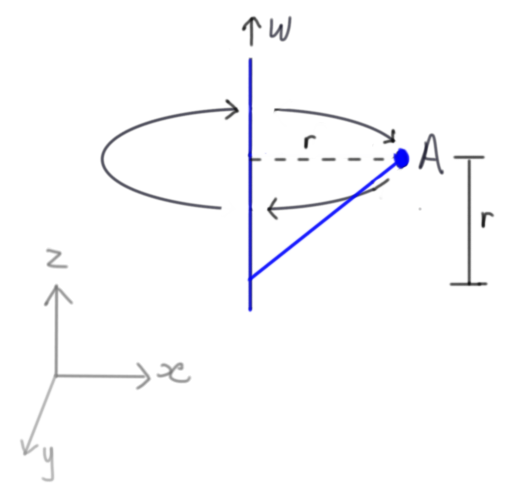
\includegraphics[height=5cm]{rod-frombelow}

\subsection*{Solution}
X = Your solution\\
Units: \si{\meter\per\second}\\
Form: Decimal, to 1 decimal place\\
Place the indicated letter in front of the number\\
Example: aX where $X=42.5$ \si{\meter\per\second} is entered as \href{http://www.wolframalpha.com/input/?i=md5+hash+of+\%22a42.5\%22}{a42.5}

$\hat{i}=$ hash of mX = b9f8f5 \si{\meter\per\second}\\
$\hat{j}=$ hash of nX = 57e394 \si{\meter\per\second}\\
$\hat{k}=$ hash of oX = 0c8b72 \si{\meter\per\second}





\newpage
\section{Radial acceleration - only direction (precession)}

\subsection*{Resources}
\begin{itemize}
    \item Book sections 7/1 to 7/5
\end{itemize}

\emph{Correction to book: Figure 7/9 should read $\bm{\alpha} = \bm{\dot{\omega}} = \bm{\Omega} \bm{\times} \bm{\omega}$ (not $\bm{\Omega} \bm{\times} \bm{r}$)}

\subsection*{Challenge}
The previous challenges considered the case (a) below, where the direction of the angular velocity vector $\omega$ was unchanging. Next consider that the angular velocity vector is precessing around an axis of symmetry, and this precession has an angular velocity of $\Omega$, as shown in (b). Combining (a) and (b) we have (c).

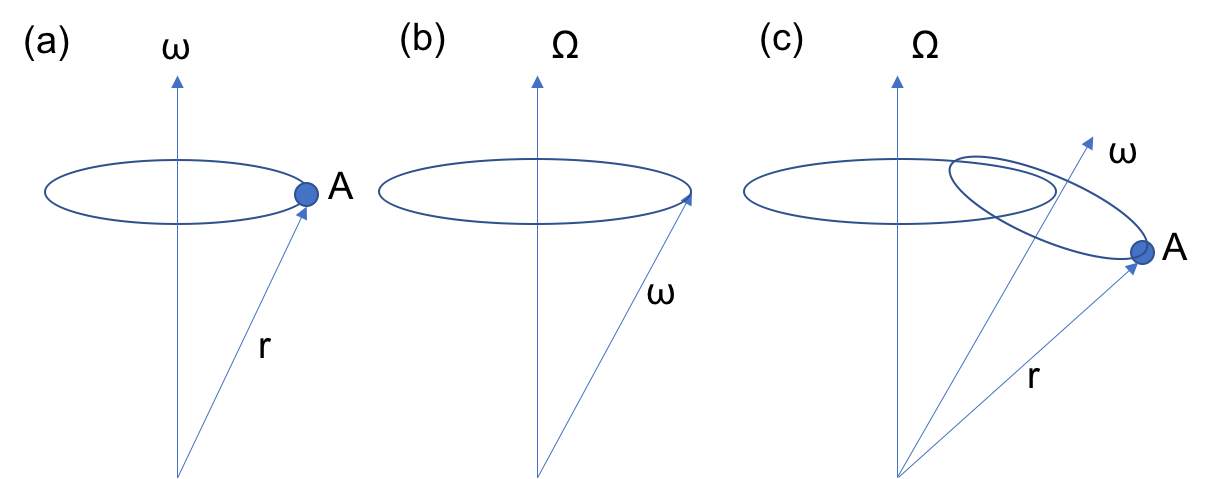
\includegraphics[height=5cm]{precession}

1. Consider the point ``A'' rotating about the vector $\omega$ with angular velocity magnitude \SI{5.5}{\radian\per\second}, but now tilt the $\omega$ vector and allow the rotation to precess around a vector of symmetry $\Omega$. Assume that only the direction (not the magnitude) of the angular velocity vector $\omega$ is changing with time. If $\Omega = 3\hat{k}$ \si{\radian\per\second} and angular velocity vector $\omega$ is inclined at \SI{45}{\degree} in the positive x-direction so that the vector $\bm{r} = 20\hat{i}$, calculate the linear acceleration of point ``A''. You may consider the origin to be at position ``A'' where the $\bm{\Omega}$, $\bm{\omega}$ and $\bm{r}$ vectors meet.

2. What is the direction of the acceleration of the angular velocity vector $\omega$? Write 1 or 2 sentences to explain why.

3. What is the direction of the linear acceleration of ``A''? Write one or two sentences (possibly with a diagram) to explain when the sign will be opposite but with same magnitude.


\subsection*{Solution}
1. $-302.5 \hat{i} + 69.15 \hat{k}$

2. and 3. Please discuss in class.




\newpage
\section{Radial acceleration II}

\subsection*{Resources}
\begin{itemize}
    \item Book sections 7/1 to 7/5
\end{itemize}

\emph{Correction to book: Figure 7/9 should read $\bm{\alpha} = \bm{\dot{\omega}} = \bm{\Omega} \bm{\times} \bm{\omega}$ (not $\bm{\Omega} \bm{\times} \bm{r}$)}

\subsection*{Challenge}
Question 7/4

\subsection*{Solution}
\SI{1285}{\meter\per\second}




\newpage
\section{Unit vector of a rotation axis}

\subsection*{Resources}
\begin{itemize}
    \item Book sections 7/1 to 7/5
\end{itemize}

\emph{Correction to book: Figure 7/9 should read $\bm{\alpha} = \bm{\dot{\omega}} = \bm{\Omega} \bm{\times} \bm{\omega}$ (not $\bm{\Omega} \bm{\times} \bm{r}$)}

\subsection*{Challenge}
Considering vector $\bm{r}$ in the figure below, if the angles $\alpha = 45$ degrees and $\beta = 30$ degrees, write the unit vector $\bm{\hat{r}}$ in terms of the Cartesian unit vectors.

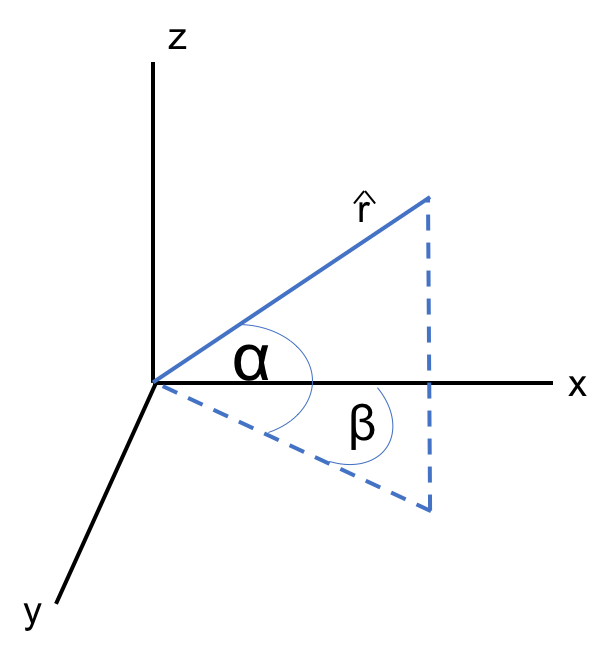
\includegraphics[height=5cm]{angles_vectors}

\subsection*{Solution}
$\bm{r} = \frac{3}{2\sqrt{2}} \hat{i} + \frac{1}{2\sqrt{2}} \hat{j} + \frac{1}{\sqrt{2}} \hat{k}$


\newpage
\section{Simultaneous rotation I}

\subsection*{Resources}
\begin{itemize}
    \item Book sections 7/1 to 7/5
\end{itemize}

\emph{Correction to book: Figure 7/9 should read $\bm{\alpha} = \bm{\dot{\omega}} = \bm{\Omega} \bm{\times} \bm{\omega}$ (not $\bm{\Omega} \bm{\times} \bm{r}$)}

\subsection*{Challenge}
Work through sample problem 7/2.




\newpage
\section{Simultaneous rotation II}

\subsection*{Resources}
\begin{itemize}
    \item Book sections 7/1 to 7/5
\end{itemize}

\emph{Correction to book: Figure 7/9 should read $\bm{\alpha} = \bm{\dot{\omega}} = \bm{\Omega} \bm{\times} \bm{\omega}$ (not $\bm{\Omega} \bm{\times} \bm{r}$)}

\subsection*{Challenge}
Work through sample problem 7/1, parts (a) and (b) only.




% NT: Add something about LH and RH systems
\newpage
\section{Simultaneous rotation III}

\subsection*{Resources}
\begin{itemize}
    \item Book sections 7/1 to 7/5
\end{itemize}

\emph{Correction to book: Figure 7/9 should read $\bm{\alpha} = \bm{\dot{\omega}} = \bm{\Omega} \bm{\times} \bm{\omega}$ (not $\bm{\Omega} \bm{\times} \bm{r}$)}

\subsection*{Challenge}
Complete question 7/12


\subsection*{Solution}
Velocity: $\frac{\pi}{8}(-4 \hat{i} - 6 \hat{j} + 3 \hat{k})$ \si{\meter\per\second}

Acceleration: $\frac{-\pi^2}{8}(25 \hat{j} + 18 \hat{k})$ \si{\meter\per\square\second}




\newpage
\section{Time-dependent rotation of vectors I}

\subsection*{Resources}
\begin{itemize}
    \item Book section 5/7
\end{itemize}

\subsection*{Comment}
A vector $\bm{r}$ may be split into its magnitude and scaler components like $\bm{r} = r_i \bm{\hat{i}} + r_j \bm{\hat{j}} + r_k \bm{\hat{k}}$. For fixed co-ordinate systems, the direction of ($\bm{\hat{i}}$, $\bm{\hat{j}}$, $\bm{\hat{k}}$) does not vary with time, so the derivatives of the unit vectors are zero. For a rotating co-ordinate system however, the derivative chain rule must be used in order to take account of the changing directions of the unit vectors.

\subsection*{Challenge}
Consider a disk that is initially flat in the x-y plane. The z-axis can be considered to point perpendicularly up from the centre of the disk. The disk then starts spinning with angular velocity depending on time $t$:
\begin{equation}
    \bm{\omega} = \omega_i Sin(2 \pi t) \bm{\hat{i}} + \omega_j Cos(2 \pi t) \bm{\hat{j}} + \omega_k t \bm{\hat{k}}
\end{equation}

You can consider the $\bm{\hat{i}}$ and $\bm{\hat{j}}$ axes to be rotating with the disk and the $\bm{\hat{k}}$ vector to always point perpendicular to the plane of the disk. 

Derive an expression for the angular acceleration $\bm{\dot{\omega}}$ of the disk as a function of time.


\subsection*{Solution}
To check your answer, substitute the following values into your final equation:
$t=1$\\
$\omega_i=10$
$\omega_j=3$
$\omega_k=2$

and you should obtain the final result

$\bm{\dot{\omega}} = (20 \pi - 6) \bm{\hat{i}} + 2 \bm{\hat{k}}$




\newpage
\section{Time-dependent rotation of vectors II}

\subsection*{Resources}
\begin{itemize}
    \item Book section 5/7
\end{itemize}

\subsection*{Challenge}
Answer question 7/27 in the book.

\subsection*{Solution}
Given in book.




%\newpage
%\section{Cross-product derivative} %NT: Move this earlier
%
%\subsection*{Challenge}
%What is the derivative of $\bm{a}(t) \bm{\times} \bm{b}(t)$ with respect to $t$?
%
%\subsection*{Solution}
%Please compare your answer with your partner and ask the teacher if you are unsure of your answer.




\newpage
\section{Relative velocity}

\subsection*{Resources}
\begin{itemize}
    \item Book section 7/6
\end{itemize}

\subsection*{Challenge}
Consider a rotating rigid body with angular velocity $\omega=\hat{k}$. Two points, ``A'' and ``B'' are chosen on the rigid body. The book describes how it is possible to calculate the velocity of point ``A'' given the velocity of point ``B''. By calculating the velocity of point ``A'' in the 3 cases below, prove that the velocity of ``A'' can be calculated accurately irrespective of choice of the location of ``B''.

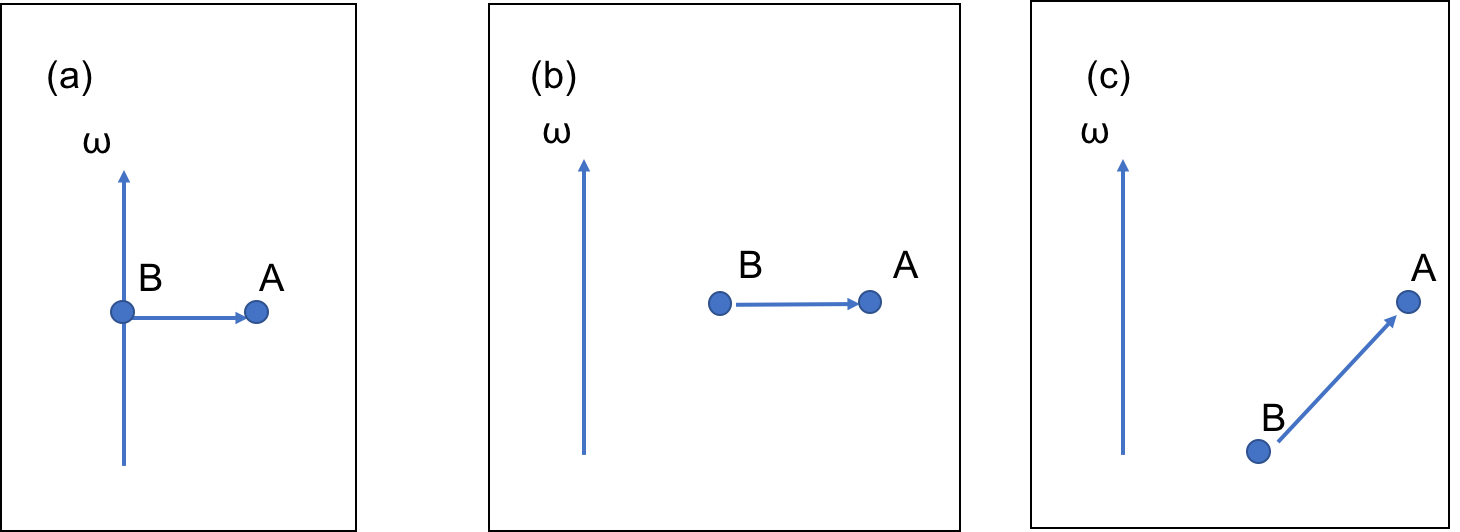
\includegraphics[width=15cm]{rigid_body_vectors}

a) $\bm{B} = \hat{k}$,              $\bm{A} = \hat{i} + \hat{k}$\\
b) $\bm{B} = \hat{i} + \hat{k}$,    $\bm{A} = 2 \hat{i} + \hat{k}$\\
c) $\bm{B} = \hat{i}$,              $\bm{A} = 2 \hat{i} + \hat{k}$

\subsection*{Solution}
You should be able to show that all 3 cases will result in the same value of $v_A$. If this is not the case, please discuss with your partner or the teacher.




\newpage
\section{Crank-style problem}

\subsection*{Resources}
\begin{itemize}
    \item Book section 7/6
\end{itemize}

\subsection*{Comment}
The angular velocity of the link $\bar{AB}$ is, by definition, perpendicular to the axis of the link. In the second part of this challenge, you use this fact along with other obtained equations to obtain the 3 Cartesian directions of the angular velocity vector. Note that although the concept of the angular momentum of the link $\bar{AB}$ is used to calculate $w_2$ in the first part of the problem, you don't actually need to calculate the value of the $\bm{w_n}$ vector in order to determine the value of $w_2$.

\subsection*{Challenge}
Work through sample problem 7/3




\newpage
\section{Perpendicular position, velocity and rotation vectors}

\subsection*{Challenge}
Prove that $\bm{r}_{AB}$, $\bm{v}_{AB}$ and $\bm{\omega}_n$ in sample problem 7/3 are all perpendicular to each other.




\newpage
\section{Perpendicular double cross-product}

\subsection*{Challenge}
Considering a vector $\bm{a} = \hat{k}$ and a vector $\bm{b} = \hat{i}$, show that $\bm{a} \bm{\times} (\bm{a} \bm{\times} \bm{b}) = -a^2 \bm{b}$.




\newpage
\section{3D acceleration}

\subsection*{Resources}
\begin{itemize}
    \item Book section 7/6
\end{itemize}

\subsection*{Comment}
In this sample problem the concept that $\bm{\dot{\omega}}_n$ is normal to $\bm{r}_{AB}$,
%but not $\bm{v}_{AB}$,
is included. ``A'' and ``B'' are part of a rigid body and therefore the separation between them is constant, even while the ijk components of $\bm{r}_{AB}$ vary with orientation of $\bm{r}_{AB}$. Despite this constant variation in orientation, angular velocity is always normal to $\bm{r}_{AB}$, by definition, because rotation parallel to $\bm{r}_{AB}$ has no influence on the motion of $\bar{AB}$. Any angular acceleration parallel to $\bm{r}_{AB}$ has no effect on the motion of $\hat{AB}$, and since the direction of $\bm{\omega}_n$ is always defined to be normal to $\bm{r}_{AB}$, the angular acceleration $\bm{\dot{\omega}}_n$ is also always normal to $\bm{r}_{AB}$.
% So you can imagine $\bm{r}_{AB}$ spinning like the propellor of an aircraft engine (relative to the $\bm{w}_n$ vector). 
%Consider a disc laying the x-y plane with the z-axis pointing up through the centre of the disc and the disc rotating with an angular velocity vector pointing directly up through the centre of the disk in the positive z-direction. Now tilt the disc so the angular velocity vector no-longer points along the z-axis, but instead precesses a vector of symettry with another angular velocity which points along the positive z-axis. The acceleration of the vector omega remains normal to the plane of the disc at all times so a point on the edge of the disc always has the same distance from the centre of the disc, however the instantanious velocity of the point on the disc depends on the precession of the vector omega.

\subsection*{Challenge}
Work through sample problem 7/4.




\newpage
\section{3D velocity calculation}

\subsection*{Resources}
\begin{itemize}
    \item Book section 7/6
\end{itemize}

\subsection*{Challenge}
Answer question 7/38.

\subsection*{Solution}
$-0.64 \hat{i} - 4.87 \hat{j} + 1.27 \hat{k}$ \si{\meter\per\second}




\newpage
\section{3D velocity and acceleration calculation}

\subsection*{Resources}
\begin{itemize}
    \item Book section 7/6
\end{itemize}

\subsection*{Challenge}
Answer question 7/43.

\subsection*{Solution}
Given in book.
